\begin{name}
	{\tenchude}
	{\tendethi}
	{\tentruong}
	{\thoigian}
\end{name}
\setcounter{ex}{0}\setcounter{bt}{0}
\TN
\Opensolutionfile{ans}[ans/ansDe3-TN1]
\begin{ex}%[Đề GHK1, Nguyễn Khuyến, Nam Định 20-21]%[0D1N1-1]
	Cho mệnh đề chứa biến $P(x)\colon$  \lq\lq $x+15 \leq x^2$\rq\rq\, với $x$ là số thực. Mệnh đề nào sau đây là đúng?
	\choice
	{$P(0)$}
	{ $P(3)$}
	{ $P(4)$}
	{\True $P(5)$ }
	\loigiai{
		Ta có $ P(5)\colon $  \lq\lq $ 5+15\le 25 $\rq\rq\, là một mệnh đề đúng.
	}
\end{ex}

\begin{ex}%[0D1H1-3]
	Viết mệnh đề phủ định $\overline P$ của mệnh đề $P$: \lq\lq Tất cả các học sinh khối $10$ của trường em đều biết bơi\rq\rq.
	\choice
	{$\overline P $: \lq\lq Tất cả các học sinh khối $10$ trường em đều biết bơi\rq\rq}
	{\True $\overline P $: \lq\lq Trong các học sinh khối $10$ trường em, có bạn không biết bơi\rq\rq}
	{$\overline P $: \lq\lq Trong các học sinh khối $10$ trường em có bạn biết bơi\rq\rq}
	{$\overline P $: \lq\lq Tất cả các học sinh khối $10$ trường em đều không biết bơi\rq\rq}
	\loigiai{
		Mệnh đề phủ định của $P$: \lq\lq Tất cả các học sinh khối $10$ của trường em đều biết bơi\rq\rq là $\overline P $: \lq\lq Tất cả các học sinh khối $10$ trường em có bạn không biết bơi\rq\rq.
	}
\end{ex}

\begin{ex}%[Đào Trung Kiên]%[121-140: Hoàng Trình]%[0D1N2-1]
	Tập hợp $A=\left\{x\in \mathbb{R}\big| 2x^2-x+1=0\right\}$ có bao nhiêu phần tử?
	\choice
	{\True $0$}
	{$1$}
	{$2$}
	{$3$}
	\loigiai{
		Phương trình $2x^2-x+1=0$ có $\Delta <0$ nên phương trình vô nghiệm trên $\mathbb{R}$.
	}
\end{ex}

\begin{ex}%[TN hóa]%[Duong Xuan Loi]%[0D1H3-3]
	Để phục vụ cho một hội nghị quốc tế, ban tổ chức huy động $35$ người phiên dịch tiếng Anh, $30$ người phiên dịch tiếng Pháp, trong đó có $16$ người phiên dịch được cả hai thứ tiếng Anh và Pháp. Hỏi ban tổ chức đã huy động bao nhiêu người phiên dịch cho hội nghị đó?
	\choice
	{\True $49$}
	{$19$}
	{$14$}
	{$65$}
	\loigiai{
		Gọi $A$ là tập hợp người phiên dịch tiếng Anh nên $n(A)=35$.\\
		Gọi $B$ là tập hợp người phiên dịch tiếng Pháp nên $n(B)=30$.\\
		Do đó $A\cap B$ là tập hợp người phiên dịch đuọc cả hai thứ tiếng Anh và Pháp nên $n(A\cap B)=16$.\\
		Ta có $n(A\cup B)=n(A)+n(B)-n(A\cap B)=35+30-16=49$.\\
		Ban tổ chức đã huy động $49$ người phiên dịch cho hội nghị.
	}
\end{ex}

\begin{ex}%[Dự án Giảng 10-11 Nhóm Toán & LaTex, Lê Minh Thiện Anh]%[0D1H3-5]
	Trong năm vừa qua, trường THPT X có $25$ bạn thi học sinh giỏi $2$ môn Văn và Toán, trong đó có $14$ bạn thi Toán và $16$ bạn thi Văn. Hỏi trường có bao nhiêu bạn thi cả $2$ môn Văn và Toán?
	\choice
	{\True $5$}
	{$7$}
	{$4$}
	{$8$}
	\loigiai{
		\textbf{Cách 1:} Sử dụng biểu đồ Ven như hình vẽ\\
		\begin{center}
			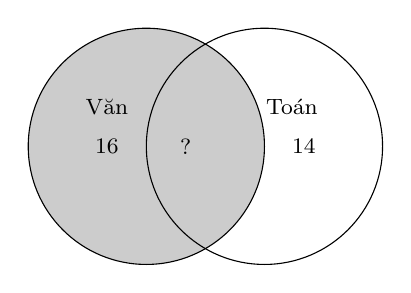
\begin{tikzpicture}[scale=1, font=\footnotesize, line join=round, line cap=round, >=stealth]
				\draw[fill=gray!40] (0,0) circle (1.5cm);
				\draw (1.5,0) circle (1.5 cm);
				\draw (-0.5,0) node {$16$};
				\draw (2,0) node {$14$};
				\draw (0.5,0) node {?};
				\draw (-0.5,0.5) node {Văn};
				\draw (1.85,0.5) node {Toán};
			\end{tikzpicture}
		\end{center}
		\noindent
		Số bạn thi toán mà không thi văn là $25-16=9$ (bạn).\\
		Số bạn thi cả $2$ môn (phần giao nhau) là $14-9=5$ (bạn).\\
		\textbf{Cách 2:}\\
		Gọi $A$, $B$ lần lượt là tập hợp các bạn thi học sinh giỏi Toán và Văn.\\
		Ta có $n(A)=14$, $n(B)=16$, $n(A\cup B)=25$.\\
		Theo công thức ta có $n(A\cap B)=n(A)+n(B)-n(A\cup B) =14+16-25=5$ (bạn).
	}
\end{ex}

\begin{ex}%[Mức độ 1]%[0D2N1-1]%[Đỗ Đường Hiếu]
	Cho bất phương trình bậc nhất hai ẩn $x+2y<3$. Cặp số nào sau đây là nghiệm của bất phương trình nói trên?
	\choice
	{$(x;y)=(1;2)$}
	{$(x;y)=(2;1)$}
	{\True $(x;y)=(1;-2)$}
	{$(x;y)=(-1;2)$}
	\loigiai{
		\begin{itemize}
			\item Thay $x=1;y=2$ vào bất phương trình $x+2y<3$ ta được $1+2\cdot 2>3$ (không thoả mãn).
			\item Thay $x=2;y=1$ vào bất phương trình $x+2y<3$ ta được $2+2\cdot 1>3$ (không thoả mãn).
			\item Thay $x=1;y=-2$ vào bất phương trình $x+2y<3$ ta được $1+2\cdot (-2)<3$ (thoả mãn).
			\item Thay $x=-1;y=2$ vào bất phương trình $x+2y<3$ ta được $-1+2\cdot 2=3$ (không thoả mãn).
		\end{itemize}
	}
\end{ex}

\begin{ex}%[0-HK1-CT-9-TranPhu-HoChiMinh-2324]%[VN-MT-6,Nguyễn Văn Minh Hiếu]%[0D2H1-2]
	\immini[thm]{Phần không gạch chéo ở hình sau đây là biểu diễn miền nghiệm của hệ bất phương trình nào trong bốn hệ A,B,C,D?
		\choice[2]
		{\True$\heva{&y>0 \\ &3 x+2 y<6.}$}{$\heva{&y>0 \\& 3 x+2 y<-6.}$}{$\heva{&x>0 \\& 3 x+2 y<6.}$}{$\heva{&x>0 \\& 3 x+2 y>-6.}$}
	}{\begin{tikzpicture}[line join=round, line cap=round, >=stealth,font=\footnotesize, scale=1]
			\fill [pattern=north east lines,pattern color=gray] (-2/3,4)--(4,4)--(4,-2) -- (10/3,-2)--cycle;
			\fill [pattern=north west lines,pattern color=gray] (-2,0) rectangle (4,-2);
			\draw[samples=100,smooth,domain=-2/3:10/3] plot(\x,{-1.5*(\x)+3});
			\draw[->](-2,0)--(4,0) node[right] {$x$};
			\draw[->](0,-2)--(0,4) node[above] {$y$};
			\node (0,0) [above left]{O};
			\fill[black] (0,3) circle (1pt) node[left]{$3$};
			\fill[black] (2,0) circle (1pt) ($(2,0)+(150:5mm)$)node{$2$};
		\end{tikzpicture}
	}
	\loigiai{Miền nghiệm của hệ bất phương trình có phần nằm phía trái trục tung $x<0$ nên loại phương án $\heva{&x>0 \\& 3 x+2 y<6}$ và $\heva{&x>0 \\& 3 x+2 y>-6.}$\\
		Miền nghiệm của hệ bất phương trình chứa điểm có tọa độ $(1;1)$ nên loại phương án $\heva{&y>0 \\& 3x+2 y<-6.}$}
\end{ex}

\begin{ex}%[0D2N2-1]%[CTST - Lớp 10 - Ôn tập cuối học kì 1 - Đề 3]%[Nguyễn Mộng Hùng]
	Hệ bất phương trình nào là hệ bất phương trình bậc nhất hai ẩn?
	\choice
	{$\heva{&0x+0y >-4\\&4x+y\ge 2}$}
	{$\heva{&2x-5y\ge 2\\&\dfrac{3}{x}-y\le-1}$}
	{$\heva{&x^2+y^3> 4\\&2x-5y\le 1}$}
	{\True $\heva{&3x+7y\le 11\\&5x-y < 5}$}
	\loigiai{
		Hệ $\heva{&3x+7y\le 11\\&5x-y < 5}$ là hệ bất phương trình bậc nhất hai ẩn.
	}
\end{ex}

\begin{ex}%[0-HK1-CT-6-HungVuong-HCM-2324]%[VN-MT-6, Nguyễn Hữu Đức]%[0D2H2-2]
	Điểm $A(1;-3)$ là điểm thuộc miền nghiệm của bất phương trình nào sao đây?
	\choice
	{\True $3x+2y<4$}
	{$2x-y<1$}
	{$x+3y>0$}
	{$-3x-y>0$}
	\loigiai{
		Ta có $3\cdot 1+2\cdot(-3)<4$ nên điểm $A$ thuộc miền nghiệm của bất phương trình $3x+2y<4$.
	}
\end{ex}

\begin{ex}%[De-chuan-hoa-so-8]%[Duong Xuan Loi]%[0H4N2-1]
	Xét tam giác $ABC$ tùy ý có $BC=a$, $AC=b$, $AB=c$. Mệnh đề nào dưới đây đúng?
	\choice
	{$c^2=a^2+b^2+2ab \cos C$}
	{\True $c^2=a^2+b^2-2 a b \cos C$}
	{$c^2=a^2+b^2+a b \cos C$}
	{$c^2=a^2+b^2-a b \cos C$}
	\loigiai{
		Theo định lí côsin ta có $c^2=a^2+b^2-2 a b \cos C$.
	}
\end{ex}

\begin{ex}%[De-chuan-hoa-so-14]%[Lê Đạt]%[0H4N2-2]
	Cho tam giác $ABC$, kí hiệu $A$, $B$, $C$ là các góc của tam giác tại các đỉnh tương ứng và $AB=c$, $AC=b$, $BC=a$. Diện tích tam giác $ABC$ bằng
	\choice
	{$S_{\triangle ABC}=\dfrac{1}{2}bc\sin B$}
	{\True $S_{\triangle ABC}=\dfrac{1}{2}bc\sin A$}
	{$S_{\triangle ABC}=\dfrac{1}{2}bc\sin C$}
	{$S_{\triangle ABC}=\dfrac{1}{2}ba\sin B$}
	\loigiai{
		Ta có $S_{\triangle ABC}=\dfrac{1}{2}bc\sin A$.
	}
\end{ex}

\begin{ex}%[0H4H2-1]
	Tam giác $ABC$ có $AB=4$, $BC=6$, $AC=2\sqrt{7}$. Điểm $M$ thuộc đoạn thẳng $BC$ sao cho $MC=2MB$. Tính độ dài đoạn thẳng $AM$
	\choice
	{$AM=4\sqrt{2}$}
	{$AM=3$}
	{\True $AM=2\sqrt{3}$}
	{$AM=3\sqrt{2}$}
	\loigiai{
	Theo định lý hàm cosin, ta có:\\
	$\cos B=\dfrac{{AB}^{2}+{BC}^{2}-{AC}^{2}}{2\cdot {AB}\cdot {BC}}=\dfrac{1}{2}$\\
	Do $MC=2MB$ nên $MB=\dfrac{1}{3}{BC}=\dfrac{1}{3}\cdot 6=2$\\
	Theo định lý hàm cosin, ta có:\\
	${AM}^{2}={AB}^{2}+{BM}^{2}-2{AB}\cdot{BM} \cdot {\cos B}=4^2+2^2-2\cdot 4\cdot2 \cdot \dfrac{1}{2}=12$\\
	Do đó $AM=2\sqrt{3}$

	}
\end{ex}

\begin{ex}%[0H4H1-2]%[Đề chuẩn hóa số 2]%[BCTuan]
	Cho tam giác $ABC$. Tính $P=\sin A\cdot \sin(B+C)-\cos A \cdot\cos (B+C)$.
	\choice
	{\True$P=1$}
	{$P=-1$}
	{$P=2$}
	{$P=0$}
	\loigiai{
		Ta có $\widehat{A}+\widehat{B}+\widehat{C}=180^\circ$, khi đó
		\begin{eqnarray*}
			P&=& \sin A\cdot \sin(B+C)-\cos A \cdot\cos (B+C)\\
			&=& \sin A\cdot \sin(180^\circ-A)-\cos A \cdot\cos (180^\circ-A)\\
			&=& \sin A\cdot \sin A+\cos A \cdot\cos A\\
			&=& \sin^2A+\cos^2A=1.\\
		\end{eqnarray*}
	}
\end{ex}

\begin{ex}%[De-chuan-hoa-so-8]%[Duong Xuan Loi]%[0H5N1-3]
	Hai véc-tơ được gọi là bằng nhau nếu chúng
	\choice
	{cùng hướng}
	{\True cùng hướng và cùng độ dài}
	{cùng phương}
	{có độ dài bằng nhau}
	\loigiai{
		Hai véc-tơ được gọi là bằng nhau nếu chúng cùng hướng và cùng độ dài.
	}
\end{ex}

\begin{ex}%[0H5N2-2]%[VN-MT6, Đào Trung Kiên]%[Sở Bắc Giang]
	Cho bốn điểm bất kì $A$, $B$, $C$, $O$. Đẳng thức nào sau đây đúng?
	\choice
	{$\overrightarrow{AB}=\overrightarrow{AC}+\overrightarrow{BC}$}
	{$\overrightarrow{OA}=\overrightarrow{OB}+\overrightarrow{AB}$}
	{\True $\overrightarrow{OA}=\overrightarrow{CA}+\overrightarrow{OC}$}
	{$\overrightarrow{AB}=\overrightarrow{OB}+\overrightarrow{OA}$}
	\loigiai
	{
		Ta có $\overrightarrow{OA}=\overrightarrow{OC}+\overrightarrow{CA}=\overrightarrow{CA}+\overrightarrow{OC}$.
	}
\end{ex}

\begin{ex}%[0H5H2-2]%[KNTT - Lớp 10 - Ôn tập cuối học kì 1 - Đề 5]%[Phạm Hải Dương]
	Cho 4 điểm $A$, $B$, $C$, $D$. Đẳng thức nào sau đây là đúng?
	\choice
	{$\overrightarrow{AB} - \overrightarrow{DC} = \overrightarrow{AC} - \overrightarrow{DB}$}
	{$\overrightarrow{AB} + \overrightarrow{CD} = \overrightarrow{AD} + \overrightarrow{BC}$}
	{$\overrightarrow{AB} + \overrightarrow{CD} = \overrightarrow{DA} - \overrightarrow{CB}$}
	{\True $\overrightarrow{AB} - \overrightarrow{DC} = \overrightarrow{AD} + \overrightarrow{CB}$}
	\loigiai{
		Ta có $\overrightarrow{AB} - \overrightarrow{DC} = \overrightarrow{AD} - \overrightarrow{CB} = \overrightarrow{AC} - \overrightarrow{BC} = (\overrightarrow{AB} + \overrightarrow{BC}) - (\overrightarrow{AD} + \overrightarrow{DC}) = \overrightarrow{AC} - \overrightarrow{AC} = \overrightarrow{0}$.\\
		Vậy $\overrightarrow{AB} - \overrightarrow{DC} = \overrightarrow{AD} + \overrightarrow{CB}$.
	}
\end{ex}

\begin{ex}%[HK1, THPT Chuyên Lương Thế Vinh - Đồng Nai, 2023-2024]%[Cao Thành Thái, 10-11EX-HK1-2324]%[0H5H3-2]
	Cho tam giác $ABC$ có $G$ là trọng tâm và $I$ là trung điểm cạnh $BC$. Đẳng thức nào sau đây là \textbf{sai}?
	\choice
	{\True $\overrightarrow{AB}+\overrightarrow{AC}=3\overrightarrow{GA}$}
	{$\overrightarrow{GA}+\overrightarrow{GB}+\overrightarrow{GC}=\overrightarrow{0}$}
	{$\overrightarrow{IB}+\overrightarrow{IC}=\overrightarrow{0}$}
	{$\overrightarrow{AB}+\overrightarrow{AC}=2\overrightarrow{AI}$}
	\loigiai
	{
		\immini
		{
			Vì $I$ là trung điểm của $BC$ nên $\overrightarrow{IB}+\overrightarrow{IC}=\overrightarrow{0}$ và $\overrightarrow{AB}+\overrightarrow{AC}=2\overrightarrow{AI}$.\\
			Vì $G$ là trọng tâm của tam giác $ABC$ nên $\overrightarrow{GA}+\overrightarrow{GB}+\overrightarrow{GC}=\overrightarrow{0}$. Thêm nữa, $\overrightarrow{AI}=\dfrac{3}{2}\overrightarrow{AG}$.\\
			Từ $\overrightarrow{AB}+\overrightarrow{AC}=2\overrightarrow{AI}$ suy ra $\overrightarrow{AB}+\overrightarrow{AC}=3\overrightarrow{AG}$.
		}
		{
			\begin{tikzpicture}[line cap=round,line join=round,font=\footnotesize]
				\def\a{3}
				\path (0:0) coordinate(B) (0:\a) coordinate(C) (55:.8*\a) coordinate(A) ($(B)!.5!(C)$) coordinate(I) ($(A)!{2/3}!(I)$) coordinate(G);
				\draw (A)--(B)--(C)--cycle (A)--(I);
				\foreach \d/\g in {A/90, B/-135, C/-45, I/-90, G/10}
				\fill (\d) circle(1pt) node[shift={(\g:.3)}]{$\d$};
			\end{tikzpicture}
		}
	}
\end{ex}

\begin{ex}%[0H5N4-1]
	%Câu 4 :
	Cho hình bình hành $ABCD$, với $AB=2$, $AD=1$, $\widehat{BAD}=60^\circ $. Tích vô hướng $\overrightarrow{AB}\cdot \overrightarrow{AD}$ bằng
	\choice
	{$-1$}
	{\True $1$}
	{$-\dfrac{1}{2}$}
	{$\dfrac{1}{2}$}
	\loigiai{
		$\overrightarrow{AB}\cdot \overrightarrow{AD}=\left| \overrightarrow{AB} \right|\cdot \left| \overrightarrow{AD} \right|\cdot \cos \left( \overrightarrow{AB},\overrightarrow{AD} \right)=AB\cdot AD\cdot \cos \widehat{BAD}=2\cdot 1\cdot \cos 60^{\circ}=1$.
	}
\end{ex}

\begin{ex}%[Mức 2]%[Dự án Giảng 10-11 Nhóm Toán & LaTex, Lê Minh Thiện Anh]%[0H5H4-2]
	Cho tam giác $ABC$. Tính tổng $\left(\overrightarrow{AB},\overrightarrow{BC}\right)+\left(\overrightarrow{BC},\overrightarrow{CA}\right)+\left(\overrightarrow{CA},\overrightarrow{AB}\right)$.
	\choice
	{$180^\circ$}
	{\True $360^\circ$}
	{$270^\circ$}
	{$120^\circ$}
	\loigiai{
		Ta có $\heva{
				&\left(\overrightarrow{AB},\overrightarrow{BC}\right)=180^\circ -\widehat{ABC}\\
				&\left(\overrightarrow{BC},\overrightarrow{CA}\right)=180^\circ -\widehat{BCA}\\
				&\left(\overrightarrow{CA},\overrightarrow{AB}\right)=180^\circ -\widehat{CAB}.}$\\
		Suy ra $\left(\overrightarrow{AB},\overrightarrow{BC}\right)+\left(\overrightarrow{BC},\overrightarrow{CA}\right)+\left(\overrightarrow{CA},\overrightarrow{AB}\right)=360^\circ $.
	}
\end{ex}

\begin{ex}%[0D8N1-1]%[Dự án đề kiểm tra Toán 10 HK2 NH23-24- Nguyễn Cường]%[Sở GD-ĐT Bắc Ninh]
	Một nhóm học sinh có $6$ bạn nữ và $5$ bạn nam. Có bao nhiêu cách chọn ra một bạn từ nhóm học sinh đó?
	\choice
	{$30$}
	{\True $11$}
	{$20$}
	{$9$}
	\loigiai{
		Số cách chọn một học sinh từ nhóm học sinh là $5+6=11$.
	}
\end{ex}

\begin{ex}%[0D8H1-3]
	Một hộp chứa $10$ quả cầu màu đỏ được đánh số từ $1$ đến $10$ và $15$ quả cầu màu xanh được đánh số từ $1$ đến $15$. Chọn ngẫu nhiên $2$ quả cầu. Hỏi có bao nhiêu cách để chọn được hai quả cầu khác màu và tổng của các số trên hai quả cầu là một số lẻ?
	\choice
	{$70$}
	{\True $75$}
	{$80$}
	{$85$}
	\loigiai{
		Để tổng của hai số là một số lẻ thì một số là số lẻ và số còn lại là số chẵn. Mặt khác, do hai quả cầu được chọn khác nhau nên ta sẽ chọn theo cách sau đây
		\begin{itemize}
			\item Chọn quả đỏ số chẵn và quả xanh số lẻ.
			      \begin{itemize}
				      \item Chọn $1$ quả cầu đỏ, có $5$ cách.
				      \item Chọn $1$ quả cầu xanh, có $8$ cách.
			      \end{itemize}
			      Trường hợp này có $5\cdot8=40$ cách.
			\item Chọn quả đỏ số lẻ và quả xanh số chẵn.
			      \begin{itemize}
				      \item Chọn $1$ quả cầu đ, có $5$ cách.
				      \item Chọn $1$ quả cầu xanh, có $7$ cách.
			      \end{itemize}
			      Trường hợp này có  $5\cdot 7=35$ cách.
		\end{itemize}
		Vậy tổng cộng có tất cả $40+35=75$ cách.
	}
\end{ex}

\begin{ex}%[BG - 10 New - 3in1, Nguyễn Văn Cường (Cường NV)]%[0D8H1-2]
	Có $3$ kiểu mặt đồng hồ đeo tay (vuông, tròn, elip) và $4$ kiểu dây (kim loại, da, vải và nhựa). Hỏi có bao nhiêu cách chọn một chiếc đồng hồ gồm một mặt và một dây?
	\choice
	{$4$}
	{\True $12$}
	{$7$}
	{$16$}
	\loigiai{
		Để chọn một chiếc đồng hồ, ta có
		\begin{itemize}
			\item Có 3 cách chọn mặt.
			\item Có 4 cách chọn dây.
		\end{itemize}
		Vậy theo qui tắc nhân ta có $3 \times 4=12$ cách.
	}
\end{ex}

\begin{ex}%[0D8N2-1]
	Cho $k,n$ là các số nguyên dương, $k \leq n$. Trong các phát biểu sau, phát biểu nào \textbf{sai}?
	\choice
	{$\mathrm{C}_n^k=\mathrm{C}_n^{n-k}$}
	{$\mathrm{C}_n^k=\dfrac{n!}{k!(n-k)!}$}
	{$\mathrm{A}_n^k=\dfrac{n!}{(n-k)!}$}
	{\True $\mathrm{C}_n^k=\mathrm{A}_n^k \cdot k!$}
	\loigiai{
		Công thức $\mathrm{C}_n^k=\mathrm{A}_n^k \cdot k!$ sai, công thức đúng phải là $\mathrm{C}_n^k=\dfrac{\mathrm{A}_n^k}{k!}$.
	}
\end{ex}

\begin{ex}%[0D8H2-3]%[Dự án đề kiểm tra Toán khối 10 HK2-NH23-24-Đợt 15-Dương Công Tạo]%[THPT Đặng Huy Trứ - Huế]
	Cho tập $A=\{1,2,3,4,5,6,7\}$. Từ tập $A$ có thể lập được bao nhiêu số tự nhiên có $3$ chữ số đôi một khác nhau?
	\choice
	{$\mathrm{C}_7^3$}
	{$P_3$}
	{$7^3$}
	{\True $\mathrm{A}_7^3$}
	\loigiai{
		Số tự nhiên có $3$ chữ số đôi một khác nhau được lập từ tập $A$ (có $7$ phần tử) là một chỉnh hợp chập $3$ của $7$ phần tử.\\
		Vậy ta có $\mathrm{A}_7^3$ số cần tìm.
	}
\end{ex}

\begin{ex}%[BG - 10 New - 4in1,Phú Thạch]%[0D8N3-2]
	Tìm hệ số của số hạng thứ tư trong khai triển biểu thức $(3x + 2y)^{4}$
	\choice
	{$81$}
	{$216$}
	{\True $96$}
	{$16$}
	\loigiai{
		Ta khai triển biểu thức như sau
		\begin{eqnarray*}
			(3x + 2y)^{4} &=& \mathrm{C}_4^0(3x)^4 + \mathrm{C}_4^1(3x)^3(2y)^1 + \mathrm{C}_4^2(3x)^2(2y)^2 + \mathrm{C}_4^3(3x)^1(2y)^3 +\mathrm{C}_4^4(3x)^0(2y)^4\\
			&=& 81x^4 + 216x^3y + 216x^2y^2 + 96xy^3 + 16y^4.
		\end{eqnarray*}
	}
\end{ex}

\begin{ex}%[BG - 10 New - 4in1,Phú Thạch]%[0D8H3-3]
	Hệ số của $x^5$ trong khai triển biểu thức $\left(- 5x - 2\right)^5$ là
	\choice
	{$625$}
	{$100\,000$}
	{$-500\,000$}
	{\True $-3\,125$}
	\loigiai{
		Số hạng chứa $x^5$ là $\mathrm{C}_5^5\cdot(-5)^5\cdot(-2)^0\cdot x^5=-3\,125x^5$.
		Hệ số của $x^5$ là $-3\,125$.
	}
\end{ex}

\begin{ex}%[0-HK1-KN-9-ChuongMyB-HaNoi-2324]%[VN-MT-6,Nguyễn Tuấn]%[0H9N1-3]
	Trong hệ tọa độ $Oxy$, cho điểm $A(2;1)$, $B(-4;-3)$. Tọa độ $\vec{AB}$ là
	\choice
	{$(1;-4)$}
	{$(2;-4)$}
	{\True $(-6;-4)$}
	{$(-2;-2)$}
	\loigiai{

	}
\end{ex}

\begin{ex}%[VN-MT-9]%[0-TK-HK1-KN-1-2425,Nguyễn Hữu Duy]%[0H9H1-3]
	Trong mặt phẳng toạ độ $Oxy$, cho điểm $A(2;-3)$, $B(3;4)$. Toạ độ điểm trung điểm của $AB$ là
	\choice
	{\True $\left(\dfrac{5}{2};\dfrac{1}{2}\right)$}
	{$(1;3)$}
	{$\left(-\dfrac{5}{2};\dfrac{1}{2}\right)$}
	{$(1;1)$}
	\loigiai{
		Ta có $M$ là trung điểm của $AB$ nên
		$\heva{&x_M=\dfrac{x_A+x_B}{2}=\dfrac{5}{2} \\&y_M=\dfrac{y_A+y_B}{2}=\dfrac{1}{2}}\Rightarrow M\left(\dfrac{5}{2};\dfrac{1}{2}\right)$.
	}
\end{ex}
\begin{ex}
	Cho hai vectơ $\vec{u}=(x;y)$ và $\vec{v}=(x';y')$. Trong các mệnh đề sau, mệnh đề nào đúng?
	\choice
	{$\vec{u}-\vec{v}=(x+x';y+y')$}
	{$\vec{u}+\vec{v}=(x-x';y-y')$}
	{\True $k\vec{u}=(kx;ky)$, với $k\in\mathbb{R}$}
	{$\vec{u}\cdot \vec{v}=(xx';yy')$}
\end{ex}
\begin{ex}%[0H9H1-4]
	Cho tam giác $ABC$ với $A(3;-1)$, $B(-4;2)$, $C(4;3)$. Tọa độ điểm $D$ để tứ giá $ABDC$ là hình hình hành là
	\choice
	{$D(-3;-6)$}
	{$D(3;-6)$}
	{\True $D(-3;6)$}
	{$D(3;6)$}
	\loigiai{Gọi tọa độ điểm $D$ cần tìm là $D(x;y)$.\\
		Vì $ABDC$ là hình bình hành nên $\overrightarrow{AB}=\overrightarrow{CD}$.\\
		Ta có $\overrightarrow{AB}=(-7;3)$, $\overrightarrow{CD}=(x-4;y-3)$.\\
		Vì $\overrightarrow{AB}=\overrightarrow{CD}$ nên ta được $\heva{&-7=x-4\\&3=y-3} \Leftrightarrow \heva{&x=-3\\&y=6.}$\\
		Vậy tọa độ điểm $D$ cần tìm là $D(-3;6)$.}
\end{ex}

\begin{ex}%[0H9N2-1]
	%Câu 8 :
	Cho hai véc-tơ $\overrightarrow{a}=\left( 4;3 \right)$ và $\overrightarrow{b}=\left( 1;7 \right)$. Số đo góc $\alpha $ giữa hai véc-tơ $\overrightarrow{a}$ và $\overrightarrow{b}$ bằng
	\choice
	{$90^{\circ}$}
	{\True $45^{\circ}$}
	{$60^{\circ}$}
	{$30^{\circ}$}
	\loigiai{
		Ta có
		\begin{eqnarray*}
			\cos \alpha &=&\dfrac{\overrightarrow{a}\cdot \overrightarrow{b}}{\left| \overrightarrow{a} \right|\cdot \left| \overrightarrow{b} \right|}
			=\dfrac{4\cdot 1+3\cdot 7}{\sqrt{4^2+3^2}\cdot \sqrt{1^2+7^2}}=\dfrac{1}{\sqrt{2}}
			\Rightarrow \alpha =45^{\circ}.
		\end{eqnarray*}
	}
\end{ex}

\begin{ex}%[0H9H2-2]
	Trong mặt phẳng tọa độ $Oxy$, cho tam giác $ABC$ có $A(3;1)$, $B(6;0)$ và $C(-1;-1)$. Tính số đo góc $A$ của tam giác $ABC$.
	\choice
	{$15^{\circ}$}
	{$60^{\circ}$}
	{\True $120^{\circ}$}
	{$135^{\circ}$}
	\loigiai{
	Ta có $\heva{&\overrightarrow{AB}=(3;-1)\\&\overrightarrow{AC}=(-4;-2)}$ suy ra $\heva{&AB=\sqrt{10}\\&AC=2\sqrt{10}.}$\\
	Do đó $\cos A=\cos(\overrightarrow{AB},\overrightarrow{AC})=\dfrac{\overrightarrow{AB}\cdot\overrightarrow{AC}}{AB\cdot AC}=\dfrac{3(-4)+(-1)(-2)}{\sqrt{10}\cdot 2\sqrt{10}}=-\dfrac{1}{2}$. Vậy $\widehat{A}=120^{\circ}$.
	}
\end{ex}
\begin{ex}%[0H5H3-5]
	Cho tam giác $ABC$ có $M$ là trung điểm của $BC$. Tính $\overrightarrow{AB}$ theo $\overrightarrow{AM}$ và $\overrightarrow{BC}$.
	\choice
	{$\overrightarrow{AB} = \overrightarrow{AM} + \dfrac{1}{2}\overrightarrow{BC}$}
	{$\overrightarrow{AB} = \overrightarrow{BC} + \dfrac{1}{2}\overrightarrow{AM}$}
	{\True $\overrightarrow{AB} = \overrightarrow{AM} - \dfrac{1}{2}\overrightarrow{BC}$}
	{$\overrightarrow{AB} = \overrightarrow{BC} - \dfrac{1}{2}\overrightarrow{AM}$}
	\loigiai{
		\immini{
			Ta có $\overrightarrow{AB} = \overrightarrow{AM} + \overrightarrow{MB} = \overrightarrow{AM} - \dfrac{1}{2}\overrightarrow{BC}$.
		}{
			\begin{tikzpicture}[>=stealth,line join=round,line cap=round,font=\footnotesize,scale=1]
				\tikzset{
				pics/tamgiacbg/.style n args={3}{
				code={
				\tikzset{
					% Khai báo độ dài cạnh va 2 goc
					declare function={a=3;goc1=70;goc2=-40;}
				}
				% Vẽ tam giác
				\path (0,0)coordinate (#1)--+(0:a)coordinate (#2)
				($(#1)!{sin(goc1)*.2}!{goc1}:(#2)$)coordinate (x)
				($(#2)!{sin(goc2)*.2}!{goc2}:(#1)$)coordinate (y)
				(intersection of #1--x and #2--y)coordinate (#3)
				;
				\foreach \pointo/\pointt in {#1/#3,#1/#2,#2/#3}{
						\draw[fill=black](\pointo)--(\pointt);
					}
				}
				}
				}
				\path
				(0,0)pic{tamgiacbg={B}{C}{A}}
				($(B)!.5!(C)$)coordinate (M)
				;
				\foreach \pointo/\pointt in {A/M}{
						\draw[fill=black](\pointo)--(\pointt);
					}
				\foreach \point/\goc in {A/90,B/190,C/-20,M/-90}{
						\draw[fill=black](\point)circle(.8pt)+(\goc:2mm)node[scale=.8]{$\point$};
					}
			\end{tikzpicture}
		}
	}
\end{ex}

\begin{ex}
	Cho hình vuông $ABCD$ cạnh bằng $2$. Điểm $M$ nằm trên đoạn thẳng $AC$ sao cho $AM=\dfrac{AC}{4}$. Gọi $N$ là trung điểm của đoạn thẳng $DC$. Tính $\vec{AB} \cdot \vec{MN}$.
	\choice
	{$\vec{AB} \cdot \vec{MN}=-4$}
	{$\vec{AB} \cdot \vec{MN}=0$}
	{\True $\vec{AB} \cdot \vec{MN}=1$}
	{$\vec{AB} \cdot \vec{MN}=-2$}
	\loigiai{
		$\vec{MN}=\vec{AN}-\vec{AM}=\vec{AD}+\vec{DN}-\dfrac{1}{4}\vec{AC}=\vec{AD}+\dfrac{1}{2}\vec{DC}-\dfrac{1}{4}\left(\vec{AB}+\vec{AD}\right)$\\
		$=\vec{AD}+\dfrac{1}{2}\vec{AB}-\dfrac{1}{4}\left(\vec{AB}+\vec{AD}\right)=\dfrac{3}{4}\vec{AD}+\dfrac{1}{4}\vec{AB}$.\\
		$\vec{AB} \cdot \vec{MN}=\dfrac{1}{4}\vec{AB}^2=1$
	}
\end{ex}

\begin{ex}%[0-HK1-KN-4-ThanhBinh-DongNa-2324]%[VN-MT-25, Phạm Ngọc Trung]%[0H9V1-4]
	Trong mặt phẳng tọa độ $Oxy$, cho hình bình hành $ABCD$ có $A(3;5)$, $B(7;2)$ và điểm $C$ thuộc trục hoành, điểm $D$ thuộc trục tung. Biết giao điểm $I$ của hai đường chéo của hình bình hành $ABCD$ có tọa độ là $(m; n)$. Tính giá trị của biểu thức $S=m+3n$.
	\choice
	{\True $11$}
	{$8$}
	{$-3$}
	{$7$}
	\loigiai{
		Mà điểm $C$ thuộc trục hoành nên $y_C=0$, điểm $D$ thuộc trục tung nên $x_D=0$.\\
		Vì $I$ là giao điểm của hai đường chéo của hình bình hành $ABCD$ nên $I$ là trung điểm của $AC$ và $BD$. Nên ta có
		\[ \heva{&2x_I=x_B+x_D\\&2y_I=y_A+y_C} \Rightarrow \heva{&2m=7\\&2n=5} \Leftrightarrow \heva{&m=\dfrac{7}{2}\\&n=\dfrac{5}{2}} \Rightarrow S=m+3n=\dfrac{7}{2}+\dfrac{15}{2}=11.\]}
\end{ex}

\TL
\begin{ex}%[0H4H2-1]
	Cho tam giác $ABC$ có $\widehat{B}=60^\circ$, $\widehat{C}=105^\circ$ và $BC=15$. Tính độ dài cạnh $AC$ (làm tròn kết quả đến hàng đơn vị).
	\loigiai{
		Ta có  \[\widehat{A}=180^\circ-\left( \widehat{B}+\widehat{C}\right)=15^\circ\]
		Theo định lý sin ta có
		\[\dfrac{BC}{\sin A}=\dfrac{AC}{\sin B}\Rightarrow AC=\dfrac{BC\cdot \sin B}{\sin A}=\dfrac{15\cdot \sin 60^\circ}{\sin 15^\circ}\approx 50.\]
	}
\end{ex}

\begin{ex}
	Tìm hệ số của $x^2$ trong khai triển nhị thức Newton $(x+\dfrac{1}{x})^4$
\end{ex}

\begin{ex}%[0D8V2-6]
	Trong mặt phẳng có bao nhiêu hình chữ nhật được tạo thành từ $6$ đường thẳng đôi một song song và $8$ đường thẳng phân biệt, đồng thời chúng vuông góc với $6$ đường thẳng song song đó?
	% \shortans{420}
	\loigiai{
		Gọi $A$ là tập hợp gồm $6$ đường thẳng đôi một song song, $B$ là tập hợp gồm $8$ đường thẳng phân biệt, đồng thời vuông góc với các đường thẳng của $A$.\\
		Mỗi hình chữ nhật được tạo thành bởi $2$ đường thẳng thuộc $A$ và $2$ đường thẳng thuộc $B$.\\
		Suy ra, số hình chữ nhật tạo thành từ các đường thẳng của $A$ và $B$ là $\mathrm{C}_6^2\cdot\mathrm{C}_8^2=15\cdot 28=420$.}
\end{ex}

\begin{ex}%[Dự án EX-10-11-Chuẩn hóa]%[Hoàng Thanh Phương]%[0H5C4-6]
	Cho hình vuông $ABCD$, cạnh bằng $a$. Gọi $E$, $F$ lần lượt là trung điểm $BC$, $CD$. Gọi $M$ là điểm thay đổi thỏa mãn $\overrightarrow{MA}\left(\overrightarrow{MC}+\overrightarrow{MD}\right)=0$. Tính giá trị lớn nhất của $MB$.
	\loigiai{
		\immini
		{
			Ta có $\overrightarrow{MA}\left(\overrightarrow{MC}+\overrightarrow{MD}\right)=0\Leftrightarrow \overrightarrow{MA}\cdot 2\overrightarrow{MF}=0$.\\
			Vậy $M$ nằm trên đường tròn đường kính $AF$.\\
			Gọi $I$ là trung điểm của $AF$. Khi đó $MB$ lớn nhất bằng $IB+R$.\\
			Ta có $AF=\sqrt{AD^2+DF^2}=\dfrac{a\sqrt{5}}{2}$, vậy $R=\dfrac{a\sqrt{5}}{4}$.\\
			Gọi $H$ là trung điểm của $AB$, ta có $\cos \widehat{HAF}=\dfrac{AH}{AF}=\dfrac{1}{\sqrt{5}}$.\\
			Suy ra $BI=\sqrt{AB^2+AI^2-2AB\cdot AI\cos \widehat{HAF}}=\dfrac{a\sqrt{13}}{4}$.\\
			Vậy $\max MB=\dfrac{a(\sqrt{13}+\sqrt{5})}{4}$.
		}
		{
			\begin{tikzpicture}[>=stealth,line cap=round,line join=round,font=\footnotesize,scale=0.7]
				\def\a{4}
				\path (0,0) coordinate (A)+(90:\a) coordinate (B)($(B)+(0:\a)$) coordinate (C)($(C)+(-90:\a)$) coordinate (D) ($(B)!.5!(C)$) coordinate (E) ($(D)!.5!(C)$) coordinate (F) ($(A)!.5!(F)$) coordinate (I) ($(B)!2!(I)$) coordinate (X)
				($(A)!.5!(B)$) coordinate (H);
				\path[name path=dt] (B)--(X);
				\draw (A)--(B)--(C)--(D)--cycle (A)--(F)--(H);
				\draw[->,blue] (A)--(E);
				\draw[->,blue] (B)--(F);
				\draw[dashed,teal,name path=dtr] let \p1=($(A)-(I)$) in (I) circle ({veclen(\x1,\y1)});
				\path[name intersections={of= dt and dtr}] coordinate (Y) at (intersection-1) coordinate (M) at (intersection-2);
				\draw[dashed] (B)--(M);
				\foreach \d/\g in {A/-90,B/90,C/0,D/-90,E/90,F/0,I/70,M/-90,H/180}
				\draw[fill=black] (\d) circle (1pt) +(\g:0.5cm) node{$\d$};
			\end{tikzpicture}
		}
	}
\end{ex}

\begin{ex}%[De-chuan-hoa-so-16]%[Mui Doan]%[0H9V1-6]
	Để kéo đường dây điện băng qua một cái hố hình chữ nhật $ABCD$ với độ dài $AB=140$ m, $AD=50$ m. Người ta dự định làm $5$ cột điện liên tiếp thẳng hàng và cách đều nhau. Cột thứ nhất nằm trên bờ $AB$ và cách đỉnh $A$ một khoảng bằng $10$ m. Cột thứ năm nằm trên bờ $CD$ và cách đỉnh $C$ một khoảng bằng $30$ m. Tính khoảng cách từ cột thứ tư đến bờ $AD$.
	% \shortans[]{$85$}
	\loigiai{
	\immini{
		Chọn hệ trục tọa độ như hình vẽ với $A(0;0)$, $B(140;0)$, $C(104;50)$, $D(0;50)$. Chọn vị trí $5$ cột điện ở $C_1$, $C_2$, $C_3$, $C_4$, $C_5$ như hình vẽ. Vì $C_1$ thuộc $AB$ và cách $A$ một khoảng cách bằng $10$m nên $C_1(10;0)$. Vì $C_5\in BD$ và cách $C$ một đoạn bằng $30$m nên $C_5(110;50)$.\\
	}
	{
		\begin{tikzpicture}[scale=0.8,>=stealth, font=\footnotesize, line join=round, line cap=round]
			\def\xmin{-1} \def\xmax{6}  \def\ymin{-1}  \def\ymax{3}
			%\draw[color=gray!50,dashed] (\xmin,\ymin) grid (\xmax,\ymax);
			\draw[->] (\xmin,0)--(\xmax,0) node [below]{$x$};
			\draw[->] (0,\ymin)--(0,\ymax) node [left]{$y$};
			\clip (\xmin,\ymin) rectangle (\xmax,\ymax);
			%%%%
			\path (0,0) coordinate (A)
			(5,0) coordinate (B)
			(0,2) coordinate (D)
			(0.5,0) coordinate (C_1)
			(5,2) coordinate (C)
			(3.5,2) coordinate (C_5)
			($(C_1)!1/4!(C_5)$) coordinate (C_2)
			($(C_1)!2/4!(C_5)$) coordinate (C_3)
			($(C_1)!3/4!(C_5)$) coordinate (C_4)
			;
			\foreach \t/\g in {A/120,B/-90,C/90,D/180,C_1/-90,C_5/90,C_2/160,C_3/160,C_4/160}{
					\draw[fill=black] (\t) circle (1pt) node[shift={(\g:7pt)},font=\scriptsize]{$ \t $};
				}
			\draw (A)--(B)--(C)--(D) (C_1)--(C_5);
		\end{tikzpicture}
	}
	\noindent Ta có $\overrightarrow{C_1C_4}=\dfrac{3}{4}\overrightarrow{C_1C_5}\Leftrightarrow 4\overrightarrow{OC_4}-4\overrightarrow{OC_1}=3\overrightarrow{OC_5}-3\overrightarrow{OC_1}\Leftrightarrow \overrightarrow{OC_4}=\dfrac{1}{4}\overrightarrow{OC_1}+\dfrac{3}{4}\overrightarrow{OC_5}.$\\ Suy ra $C_4(85;37{,}5)$, do đó $AD$ cách cột điện thứ $4$ cách bờ $AD$ một khoảng bằng $85$ m.
	}
\end{ex}
\Closesolutionfile{ans}
